\documentclass{article}
\usepackage{listings}
\usepackage{xcolor}
\usepackage{graphicx}
\usepackage{siunitx}
\usepackage{float}
\usepackage{setspace}
\usepackage{makecell}
\usepackage{gensymb}
\usepackage{url}

\title{N76E003 Reflow Oven Controller}
\author{Team A9}
\date{March 1st, 2024}

\definecolor{codegreen}{rgb}{0,0.6,0}
\definecolor{codegray}{rgb}{0.5,0.5,0.5}
\definecolor{codepurple}{rgb}{0.58,0,0.82}
\definecolor{backcolour}{rgb}{0.95,0.95,0.92}

\lstdefinestyle{mystyle}{
    backgroundcolor=\color{backcolour},
    commentstyle=\color{codegreen},
    keywordstyle=\color{magenta},
    numberstyle=\tiny\color{codegray},
    stringstyle=\color{codepurple},
    basicstyle=\footnotesize\ttfamily,
    breakatwhitespace=false,
    breaklines=true,
    captionpos=b,
    keepspaces=true,
    numbers=left,
    numbersep=5pt,
    showspaces=false,
    showstringspaces=false,
    showtabs=false,
    tabsize=2
}

\linespread{1.6}

\lstset{style=mystyle}

\begin{document}

\maketitle
\begin{center}
Course: ELEC 291/292 Electrical Engineering Design Studio I \\
Section: L2A \\
Instructor: Dr. Jesus Calvino-Fraga \\
\end{center}

\begin{tabular}{|c|c|c|c|}
  \hline
  Student \# & Student Name & \%Points & Signature \\
  \hline
  67286750 & Tomaz Zlindra & TBA &  \\
  \hline
  21475330 & Martin Lieu & TBA &  \\
  \hline
  7106221 & Muntakim Rahman & TBA &  \\
  \hline
  76029933 & James Huang & TBA & \\
  \hline
  17542499 & Emile Jansen  & TBA & \\
  \hline
  46634911 & Kyden McCaskill & TBA & \\
  \hline
\end{tabular}

\newpage

\tableofcontents

\newpage
\section{Introduction}

\subsection{Objective}

The objective of this project was to design, program, and test a reflow oven controller whose purpose is to be able to safely and reliably  assemble surface mounted devices to printed circuit boards. The design of this project is built upon the concepts explored in labs 1-3 including LCD interfaces, PUSH buttons, timers, ADC converters for reading external inputs such as temperature, and a serial communication interface. In addition to these concepts,  voltage amplIfiers and PWM peripherals were also used to meet our design needs.  \\

\noindent The intended outcome of this project was to leverage the limited capabilities of the N76E003 microcontroller to solder EFM8 boards for the second half of the course. Below is a picture of the breadboard we used to develop our controller.

\begin{figure}[H]
        \centering
        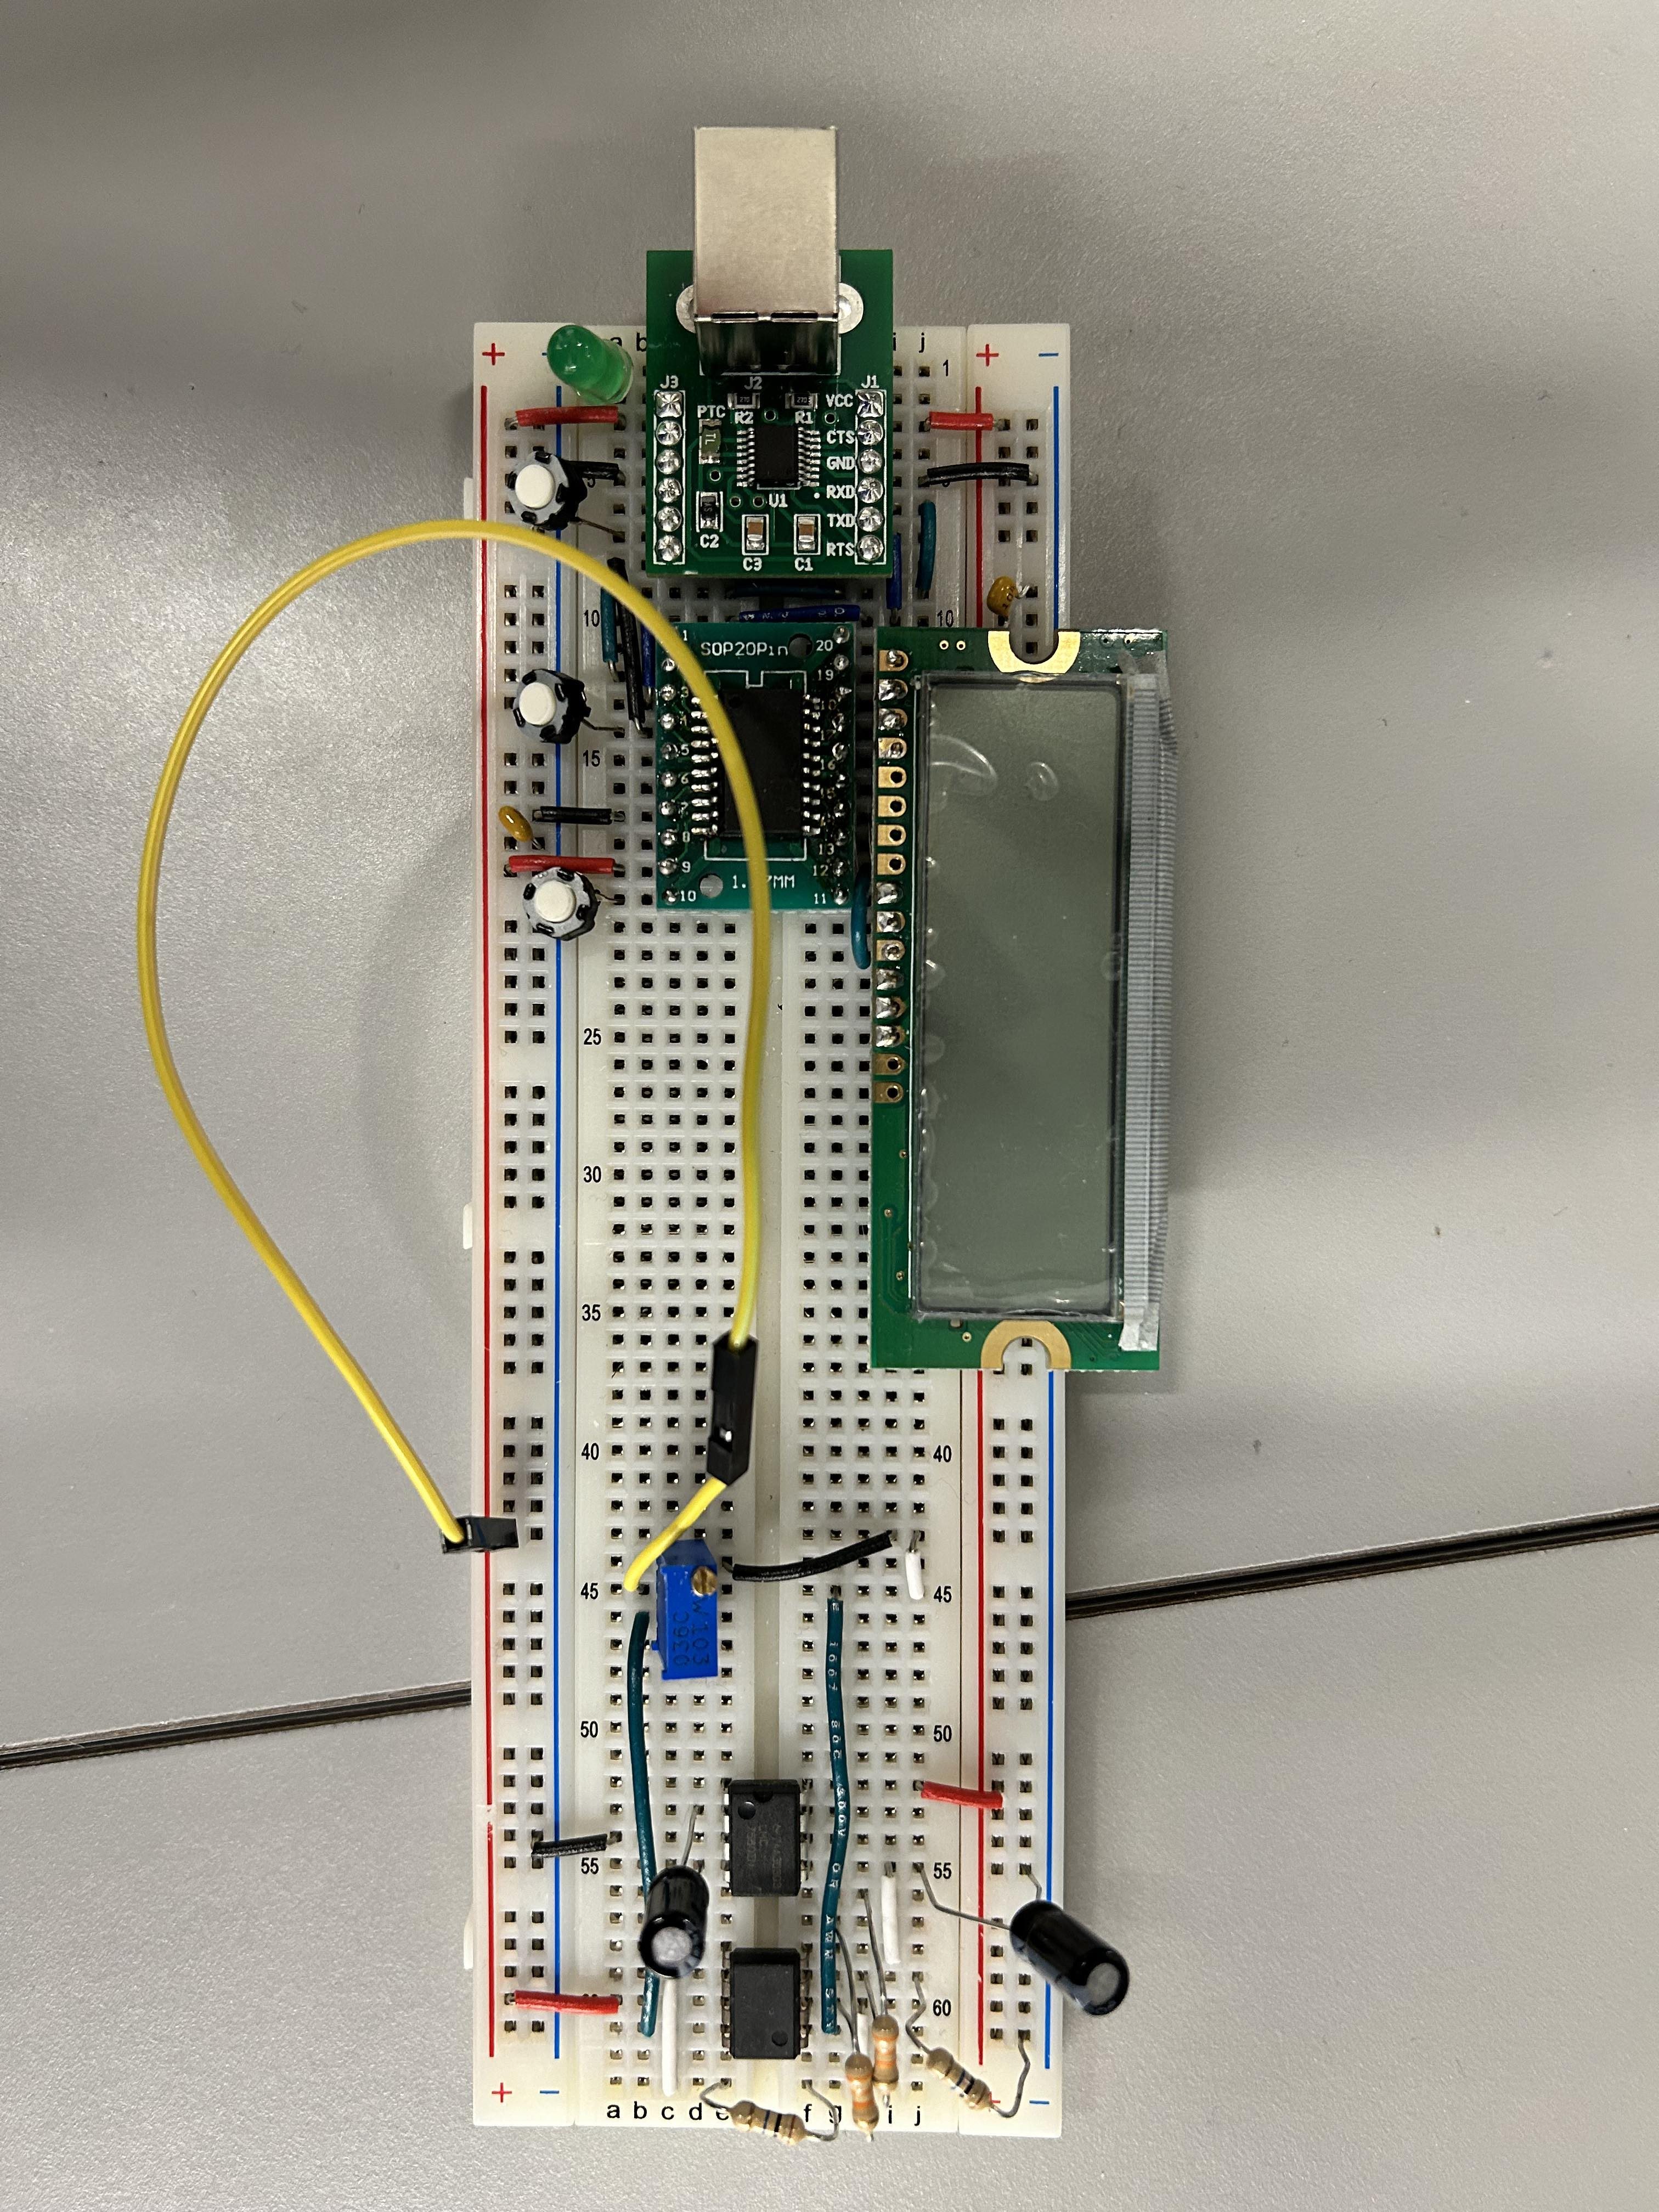
\includegraphics[width=0.4\linewidth]{Figures/CircuitOfInterest.jpg}
        \caption{Circuit of Interest}
        \label{fig:breadboard}
\end{figure}

\subsection{SpecIfications}
The tables below contain the hardware and software spefications of this project.

\begin{table}[h]
  \centering
  \begin{tabular}{|c|m{4.5cm}|m{3.5cm}|}
    \hline
    Circuit & \makecell{Chips} & \makecell{Other Components} \\
    \hline
    Main & \makecell{N6E003 Micro-Controller\\ BO230XS USB adapter} & \makecell{N/A} \\
    \hline
    Voltage AmplIfier & \makecell{OP07CP Op-Amp \\ LMC7660 Voltage Converter} & \makecell{2x 10M\ohm resistors \\ 2x 33k\ohm resistors \\ 2x 10uf capacitors \\ 1x potentiometer} \\
    \hline
    Temperature Sensing & \makecell{LM335 Temperature Sensor} & \makecell{K - Thermocouple \\ 1x potentiometer \\ 2k\ohm resistor}\\
    \hline
    PWM & \makecell{N/A} & \makecell{2N3904 Transistor \\ 1x 330\ohm resistor}\\
    \hline
    Multiplexer & \makecell{N/A} & \makecell{5x PUSH buttons\\5x 1N4148 diodes}\\
    \hline

  \end{tabular}
  \caption{Hardware SpecIfications}
  \label{tab:HardSpecs}
\end{table}

\begin{table}[h]
    \centering
    \begin{tabular}{|m{6cm}|m{6cm}|}
        \hline
         \makecell{Assembly} & \makecell{Python} \\
         \hline
         \makecell{UI on LCD\\Settable Soak time and temperature\\Settable Rise time and temperature\\Temperature calculations from ADC\\Transmit Temperature to Serial\\Transmit State to Serial and UI} & \makecell{Strip chart of Temperature Data\\Date Time IdentIfied\\ CSV Data\\ CSV File Cloud Upload}\\
         \hline

    \end{tabular}
    \caption{Software SpecIfications}
    \label{tab:SoftSpecs}
\end{table}

\subsection{Block Diagram}
The figure below contains a block diagram showing the flow of information of both hardware and software in our design.

\begin{figure}[H]
        \centering
        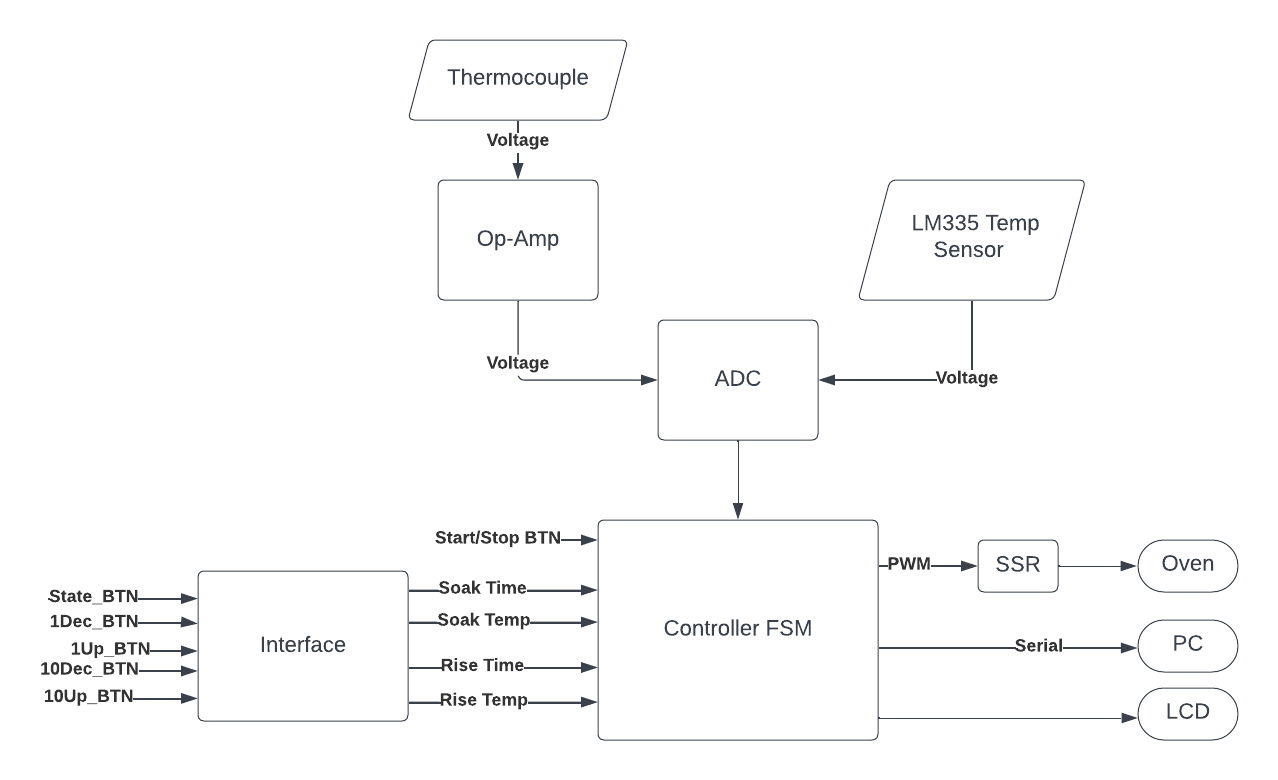
\includegraphics[width=0.6\linewidth]{Figures/Flow Chart.png}
        \caption{Block Diagram}
        \label{fig:Block Gram}
\end{figure}


\section{Investigation}

\subsection{Idea Generation}
Our idea generation process began with a thorough discussion of the individual requirements of a fully-functional controller. We then dissected the problem into smaller, manageable parts, enabling effective task allocation for firmware and hardware design. Initially, we developed individual components in isolated test environments to confirm details, such as the functionality of the ADC and PWM peripherals, the performance of the op-amp circuit, and the intended state changes. Integrating these functional components into a single, cohesive product was the final step, allowing us to fine-tune initial designs collaboratively through end-to-end testing

\subsection{Investigation Design}
In the investigation design phase, we utilized circuit simulation programs like LTspice to test the feasibility of hardware components such as the op-amp prior to manual construction. LTspice provided a platform for designing, altering, and simulating the op-amp values to meet specIfications. Additionally, we archived our past experiments on a Google Cloud server, enabling remote access to previous experimental data. This ensured that team members could generate graphs and analyze data, maintaining up-to-date knowledge.

\subsection{Data Collection}
 The ADC and temperature data collection and analysis were conducted through a three-way analytical approach using the oven. Firstly, the "kconvert" script facilitated a comparative analysis between numerical readings and actual temperatures, allowing for precise calibration. Subsequently, a custom-designed strip chart application illustrated the data, facilitating the assessment of consistency against expected patterns. Lastly, upon completion of the task, all temperature readings were uploaded and logged onto a Google Cloud server, providing a record of timestamps and temperatures for future reference and analysis.

\

\noindent Furthermore, the utilization of instruments such as an oscilloscope facilitated the examination of PWM implementation behavior, guaranteeing adherence to specIfications. After verIfying the desired functionality, we integrated the signal into our finite state machine, allowing joint observation across states to ensure continued compliance with specIfications.

\subsection{Data Synthesis}
Initial data was obtained through trial runs. It was imperative that appropriate temperatures were reached or maintained during and throughout critical stages such as state transitions or holding periods. To align graphical representations with desired diagrams, modIfications to the PWM signal were made to strengthen or weaken power output, ensuring graphical congruence. Once power optimization met specIfications, further data synthesis proceeded.

\subsection{Analysis of Results}
In analyzing results, we validated our measurements and conclusions to the degree of error and limitations illustrated by example test programs and charts. This process involved scrutinizing data for precision and accurate while considering discrepancies in trial runs.

\section{Design}

\subsection{Use of Process}
To understand the complex challenges needed to be addressed, we created a dataflow diagram of our system to understand the state changes as we progress through both
successful and unsuccessful reflow cycles. This was a key step in understanding the requirements of the project and what we must consider in our solution.

\begin{figure}[h]
        \centering
        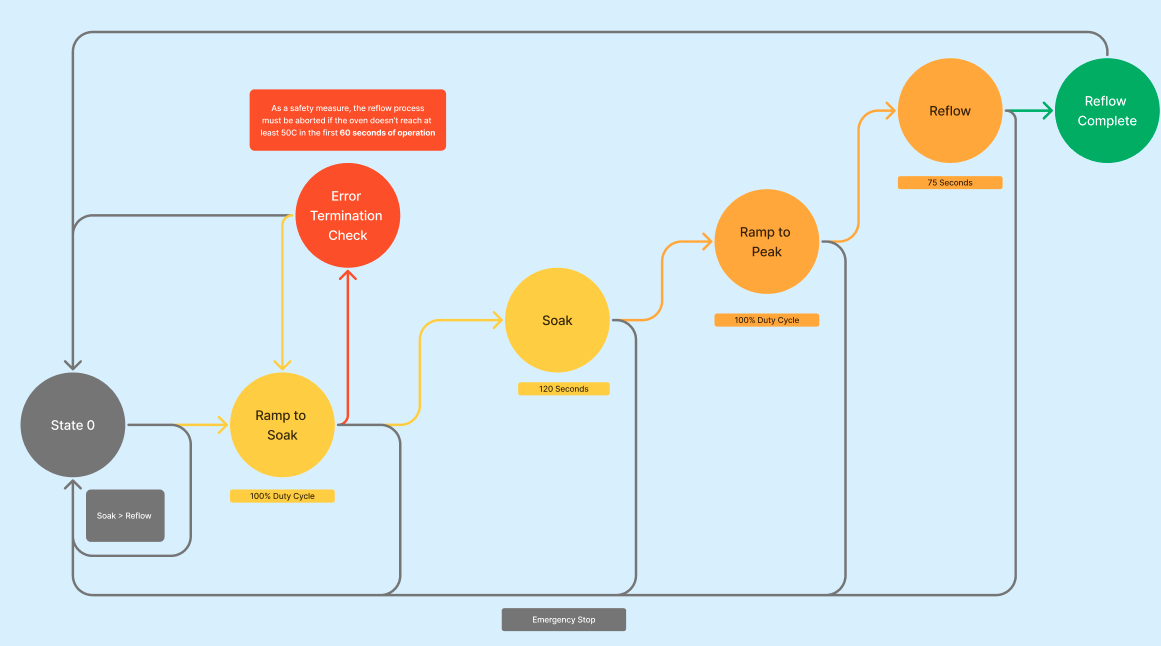
\includegraphics[width=1\linewidth]{Figures/Statemachine.png}
        \caption{Finite State Machine Diagram}
        \label{fig:Statemachine}
\end{figure}

This diagram allowed our group to determine the conditions which changed the state and the code which needed to be done once versus iteratively.

\subsection{Need and Constraint IdentIfication}
To identIfy needs for a functional oven controller, we listed functionalities expected of fully functional Reflow Oven Controller.
The main requirements for this project include the following:
\begin{itemize}
  \item Must be written in 8051 Assembly.
  \item Must measure temperatures $25^\circ\text{C} \leq T \leq 250^\circ\text{C}$, accurate to within $3^\circ\text{C}$.
  \item Must include editable soak and reflow temperatures.
  \item Must include safety features, in particular automatic cycle termination on error.
  \item Must include button functionality for initiating and terminating the reflow process.
  \item Must include an LCD Display with configuration and current temperature readings.
  \item Must communicate with a Software UI via serial communication and transmit temperature data.
\end{itemize}
Note : These were listed in a requirement PDF provided by Dr. Jesus Calvino-Fraga. \\

\noindent In addition to these, we also identIfied constraints that would affect the design of the controller. These include:
\begin{itemize}
  \item The N76E003 microcontroller has a limited number of pins, timers, and peripherals.
  \item Assembly language is not as intuitive as higher-level languages and can easily become complex in collaboration.
\end{itemize}

\noindent To get around these, we tried to start of with simplIfied functionality and iterate on it to progress towards meeting project requirements.
We collaborated via a Github repository for source control and keeping track of iteration. This allowed us to move fast on functionality, such as
the finite state machine, and then iterate on it to add more features, such as the temperature sensor and the serial communication interface.

\subsection{Problem SpecIfication}

It's become evident throughout this project that an initial listing of problems is a strong foundation for development. However,
often we have found that there are hidden problems in feature development. In summary, individual functionality of hardware and firmware modules did not
guarantee smooth integration. Collaboratively stepping through the process of reflow soldering with our prototype ensured we addressed key points, including the
planned state change and cycle termination functionality, the intended conversion of ADC readings from the K-type thermocouple voltage, and the consideration of
arithmetic operations between temperature variables.

\subsection{Solution Generation}

We found that the best way to develop our solution was in a 4 step process.

\begin{enumerate}
  \item Discussing individual requirements and assigning development to team members.
  \item Developing submodules in a test environment.
  \item Integrating the submodules into a single, cohesive product.
  \item Exhaustively test and debug functionality until requirements are met.
\end{enumerate}

\noindent Tackling the problems in the section above in a collaborative manner allowed us to address them comprehensively and is a direct contributor
to our final product. We also found that ownership over individual subcomponents allowed us to have team members who best understood particular behaviors.
When we encountered problems, we raised concerns and asked questions to move towards fixing and integrating them. \\

\noindent One issue which arose during development was the need to have distinct ADC functionality for the K-type thermocouple and the LM335 temperature sensor.
We initially tried to have identical ADC functionality for both, but this was not feasible due to the dIfferent voltage ranges and the need for additional conversion of
the thermocouple voltage to temperature. We resolved this through incremental changes and testing on our LCD. In order to ensure our firmware wasn't a black box, we printed
debugging information to the LCD. This was a makeshIft solution to being unable to halt the microcontroller and step through the code in a debugger.

\subsection{Safety/Professionalism}

To ensure our product was safe, we placed emphasis on accurate temperature reading and transmission. Once we had a semi-functional ADC module, we tested the calculated temperature
with the multimeter program provided by Dr. Jesus Calvino-Fraga. This allowed us to ensure that the temperature readings were accurate to within $3^\circ\text{C}$. In addition, the
cycle termination functionality was key to halting a faulty reflow process. This both allowed us to turn off the oven and lower temperatures, as well as to prevent damage to our EFM8 boards. Furthermore,
we added additional functionality to prevent configuration of reflow temperature below the soak temperature. This feedback was displayed to the user on the LCD.
To ensure professionalism, we maintained a clean and organized codebase, and we also maintained a professional attitude in our communication and collaboration.

\subsection{Detailed Design}

\subsubsection{Firmware Design}

Our final state machine helped us integrate submodules for the PWM, ADC, and serial transmission. In the figure below, it is noticed that our firmware peripherals send datastreams directly to the serial port and the LCD. For arithmetic operations in our Math modules, we use hexadecimal variables and this is sent to our Python software application for data post-processing. The LCD, however accesses a Binary Coded Decimal copy of our calculated temperature. This is to prevent the complications of $bcd2hex$ operations in our arithmetic. We decided it was simpler and a more straightforward solution to have dedicated variables for these separate datastreams.

\begin{figure}[H]
  \centering
  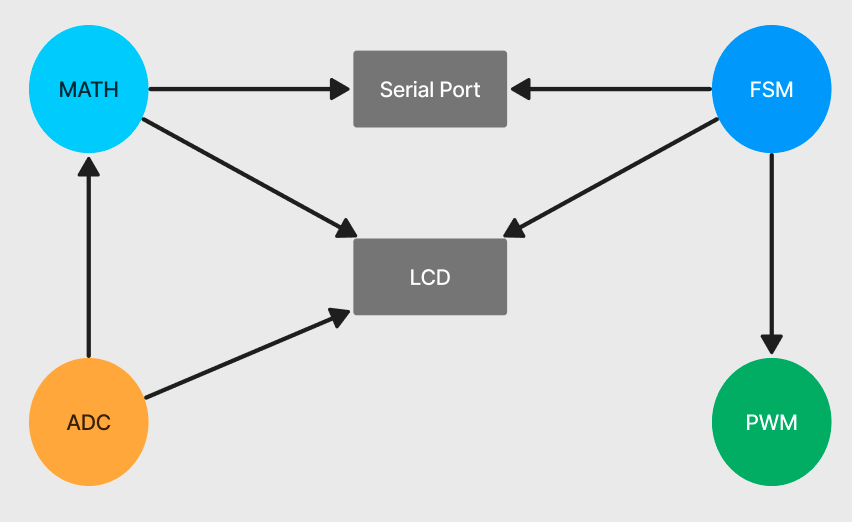
\includegraphics[width=0.8\linewidth]{Figures/Software_Modules.png}
  \caption{Software Modules Diagram}
  \label{fig:Software Modules}
\end{figure}

\noindent From discussing the slow response time of the oven, we decided to implement a $1s$ PWM period.

The ADC was set to store data in 4 byte variables. These were offset to ensure we add the correct digits from the thermocouple temperature and the LM335 temperature sensor.

\begin{lstlisting}[language={[x86masm]Assembler}]
Get_THERMOCOUPLE_TEMP:
	; Read AIN7 on Pin 14
	ANL ADCCON0, #0XF0
	ORL ADCCON0, #0X07 ; Select ADC Channel 7
	LCALL Read_ADC_Avg
	LCALL Convert_Voltage
Calculate_THERMOCOUPLE_TEMP:
	LCALL hex2bcd
	MOV Output_Voltage+3, BCD+3
	MOV Output_Voltage+2, BCD+2
	MOV Output_Voltage+1, BCD+1
	MOV Output_Voltage+0, BCD+0

	Load_y(1000) ; Vout * 1000 / 12424
	LCALL mul32
	Load_y(12424)
	LCALL div32
	Load_y(100)
	LCALL mul32

	; Save Result to Use Later.
	MOV THERMOCOUPLE_TEMP+3, X+3
	MOV THERMOCOUPLE_TEMP+2, X+2
	MOV THERMOCOUPLE_TEMP+1, X+1
	MOV THERMOCOUPLE_TEMP+0, X+0

	RET
\end{lstlisting}

\noindent As mentioned previously, we store a BCD copy of our calculations for the LCD. This is stored in 2 bytes as shown below.

\begin{lstlisting}[language={[x86masm]Assembler}]
Write_Oven_BCD:
	MOV X+0, OVEN_TEMP
	MOV X+1, #0
	MOV X+2, #0
	MOV X+3, #0

	LCALL hex2BCD
	MOV OVEN_BCD+1, BCD+1
	MOV OVEN_BCD+0, BCD+0

	RET
\end{lstlisting}

Our calculated oven temperature was stored in 1 byte. This was due to our interest in integer values between $25^\circ\text{C}$ and $250^\circ\text{C}$.

\begin{figure}[H]
  \centering
  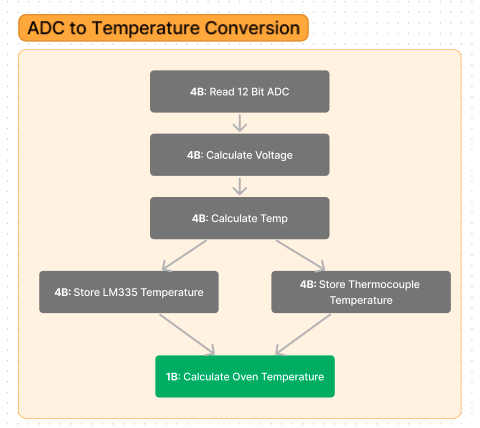
\includegraphics[width=0.8\linewidth]{Figures/ADC.png}
  \caption{ADC Dataflow Diagram}
  \label{fig:ADC}
\end{figure}

\noindent To compare the current oven temperature with the 1 byte reflow and soak temperatures, we used the 8051 assembly compare instruction. This allowed us to set flags for the state machine to progress through the reflow cycle.

\begin{lstlisting}[language={[x86masm]Assembler}]
  Below_Temp_Flag: DBIT 1 ; For State Changes
  Error_Triggered_Flag: DBIT 1 ; For Cycle Termination
  ...
  Reflow_Soak_Flag:   DBIT 1 ; For State Changes
  State_TX_Flag: DBIT 1 ; For Serial Transmission of State Number
\end{lstlisting}

\noindent We also applied this same flag logic to the serial transmission of the state number. This allowed us to transmit the state number to the software UI and to the LCD.
This enabled us to overcome the problem of having a datastream dominated by state numbers rather than relevant temperature data. Instead we used this flag during state changes to transmit this to the software UI.

With this design, we are able to achieve data reliability in our data post-processing as shown in the $csv$ data graphed below.

\begin{figure}[H]
  \centering
  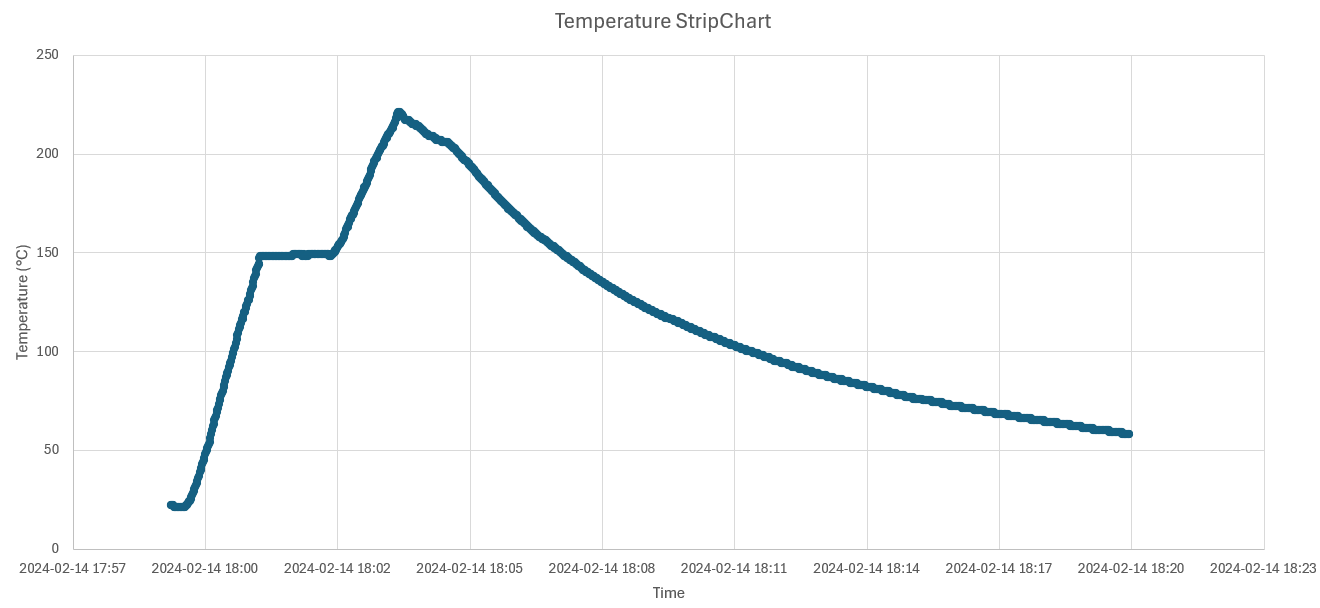
\includegraphics[width=1.0\linewidth]{Figures/Reflow_Data.png}
  \caption{Reflow Data}
  \label{fig:Reflow Data}
\end{figure}

\subsection{Solution Assessment}

\noindent We assessed our design from a set of tests. Initially, before we had a working version of the controller, we would first test the FSM, ADC conversions, PWM, OP Amp circuit and Serial seperately (typically by having an assembly file which would simulate it). Once we knew each module was working individually, we integrated them one by one, testing them completely before adding the next module. To validate whether our system worked, we would use electrical tools such as oscilloscopes, multimeters and of course, the LCD display. Most of these systems were debugged by using a test-and-try procedure.

\

\noindent Below is a brief overview of how we debugged certain systems:
\begin{itemize}
\item FSM. This was debugged by displaying the state number, the timer and the resulting timer counter on the LCD, with a button to change state when in a non-timer state.
\item PWM. This was debugged by displaying the wave onto the oscilloscope, and viewing the shape and period of the square wave.
\item ADC. This was debugged by displaying the full thermocouple and room temperatures on the LCD, and ensuring the addition is correct.
\item OP Amp. This was simply debugged by ensuring proper wiring, simultating on LTSpice, and finally using the multimeter to obtain the voltage readings.
\end{itemize}

\

\noindent To validate our oven temperature data, we used a python script provided by Dr. Calvino-Fraga, which would directly convert the voltage dIfference across the thermocouple into temperature. When our design was complete, we let our controller progress through the reflow process, comparing the dIfference of the temperature sent over serial versus the one displayed by the script. After some fine tuning of the op amp amplIfication calculations and implementing a 0 offset on the op amp, we noticed the temperature dIfference was never more than 2 degrees celcius. The temperature dIfference seemed larger than expected due to having only 3 signIficant figures (0 decimal places) being sent over by the serial port. We were also able to display the temperature on the python graph, to see the live temperature as shown in Figure \ref{fig:Reflow Data}. This allowed us to modIfy the duty cycle of the PWM signal to ensure the reflow and soak states remain approximately the right temperature.

\

\noindent Our design has many strengths and weaknesses. The strengths include:
\begin{itemize}
    \item Reliable data. The data shown by the serial port was always identical to the one displayed on the LCD, and never spiked due to secure hardware connections.
    \item Deterministic state transitions. We studied the state transitions extensively with plenty of individual testing early in the design process.
    \item Safety features, including the cycle termination functionality and the configuration handling of the soak and reflow temperatures.
\end{itemize}
Unfortunately, this design also has many weaknesses, such as:
\begin{itemize}
    \item Used excessive breadboard space. The controller was placed on two breadboards, which requires more connections and visually appears more bulky.
    \item Ameliorated temperature accuracy. Although our data was approximately 1-2 degrees celsius off from the real temperature, this should've been more accurate.
    \item Codebase requires refactoring to be more transparent. Submodules can appear as a black box If accessed by new individuals (e.g. ADC arithmetic). Variable names require more clarity and should follow standard naming convention. Codebase maintainability was benefited from migrating most submodule logic to dedicated $.inc$ files. This should be continued to ensure the $fsm.asm$ file includes only high level logic (i.e. only include function calls).
\end{itemize}

\noindent We believe, with more emphasis on these issues, these weaknesses could've been addressed.

\section{LIfe Long Learning}
Through this project, we gained valuable experience that would help us grow in our respective fields of engineering. We initially encountered challenges when using assembly language to create the basic features, due to our relative lack of experience with it. We also encountered challenges with signal data processing and attempting to send and receive data through the serial port.

\

\noindent On the hardware side of things, we had to learn how to assemble op-amp circuits and multiplex systems that would be important to our final product. We were able to use and expand upon the programming knowledge we learned in ELEC 291, CPSC 259, and CPEN 211 to program the necessary modules needed to meet the requirements. Through collaboration, cooperation, and communication, we were able to integrate multiple hardware and firmware modules into a single, cohesive product. Utilizing the oscilloscope and multimeter, we were able to successfully perform signal processing and validate our design.

\

\noindent Additionally, we were able to delve into data post-processing and object-oriented software development in our Python applications. We applied the networking principles from ELEC 331 as well in our
automation with the cloud server.

\section{Conclusions}
By the end of the project, we were able to develop a fully functional reflow oven controller. With it, could control the temperature of the oven to use the reflow soldering method to assemble the EFM8 boards needed for Labs 4 and 5. In addition, we explored additional engineering principles in our feature development. This controller will serve as a strong foundation for future projects and was a great learning experience for our team.

\section{References}
\begin{itemize}
  \item OP07C Data sheet Texas Insturments: \url{https://www.ti.com/product/OP07C}
  \item LMC7660 Data sheet Texas Instruments: \url{https://www.ti.com/product/LMC7660}
  \item LM335 Data sheet Texas Insturments: \url{https://www.ti.com/product/LM335}
  \item 2N3904 Data sheet ON semi: \url{https://www.onsemi.com/pdf/datasheet/2n3904-d.pdf}
\end{itemize}
\section{Bibliography}
\section{Appendices}

\end{document}